In order to execute vector operations, hardware needs to align data in vector
registers, e.g. XMM0, YMM0 or ZMM0 for x86 architectures. Moving data between
memory and registers, or registers and registers, has, of course, a cost,
in most cases difficult to measure and quantify due to data races in code,
cache complexity, out-of-order engines, port decoding occupancy, frequency
scaling, among others. Compilers may generate different instructions for
different architectures using the same ISA (e.g. AVX2), according to a model.
From stated above, it is difficult to create an accurate estimation or cost
model, which can be defined as the computation of the total cost of a certain
region.

\begin{figure*}[ht]
	\centering
	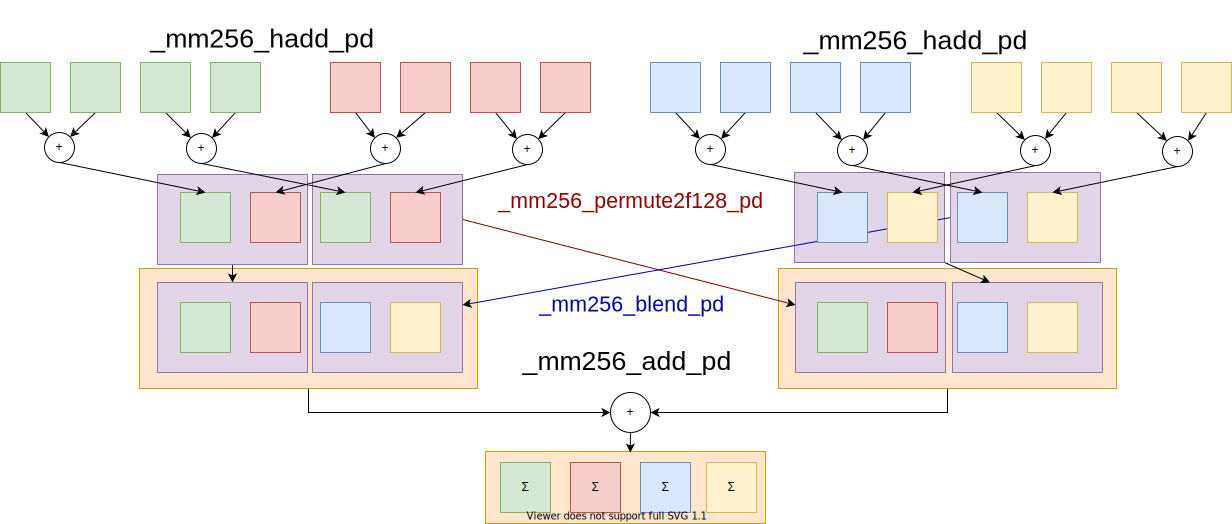
\includegraphics[width=\textwidth]{img/FusedReductions.pdf}
	\caption{}
	\label{fig:FusedReductions}
\end{figure*}